\chapter{سخت‌افزار ربات}
\section{مقدمه}
در این قسمت از پایان نامه، به بررسی اجزای اساسی ربات‌ها می‌پردازیم. این اجزا شامل سروموتورها، میکروکنترلرها، بردهای الکترونیکی و سایر قطعات مهم می‌شوند که در ساخت و کنترل ربات‌ها به کار می‌روند. این اجزا با تعامل و همکاری با یکدیگر، امکان حرکت، حسگری و کنترل دقیق را برای ربات‌ها فراهم می‌کنند. در ادامه به بررسی عمیق‌تر هر یک از این اجزا خواهیم پرداخت و نقش آنها در عملکرد کلی ربات‌ها را بررسی خواهیم کرد. همچنین، اهمیت انتخاب و استفاده صحیح از این اجزا را نیز بررسی می‌نماییم. این مقدمه به ما امکان می‌دهد تا به دنیای پیچیده و هیجان‌انگیز رباتیک در عمق بپردازیم و راهنمایی کنیم. 
\section[سرو موتور]{سرو موتور\cite{Servo}}
سروموتورها از جمله اجزاء اساسی در رباتیک و به‌ویژه در ربات‌های چهارپا مورد استفاده قرار می‌گیرند. این اجزا جهت کنترل و حرکت اندام‌ها و پاهای ربات به کار می‌روند. سروموتورها معمولاً دارای یک شفت قابل چرخش هستند که از طریق یک سیگنال کنترلی به جلو و عقب حرکت می‌کنند. سروموتورها به دلیل دقت، سرعت و کاربرد‌های متعددشان، بخش مهمی از طراحی و ساخت ربات‌های چهارپا را تشکیل می‌دهند.

در ربات‌های چهارپا، سروموتورها به‌عنوان موتورهای اصلی برای حرکت پاها و اندام‌ها عمل می‌کنند. این سروموتورها معمولاً دقیق و قابل کنترل با سرعت متغیر هستند، که این ویژگی‌ها امکان جابه‌جایی دقیق و پیچیده را فراهم می‌کنند. سروموتورها معمولاً با استفاده از میکروکنترلرها به راحتی کنترل می‌شوند. این اجزا به تنهایی یا به صورت گروهی در ربات‌های چهارپا استفاده می‌شوند تا حرکت و موقعیت دقیق در سیستم رباتیک تضمین شود.
 
    \begin{figure}[!h]
	\centering
	\vspace{1cm}
	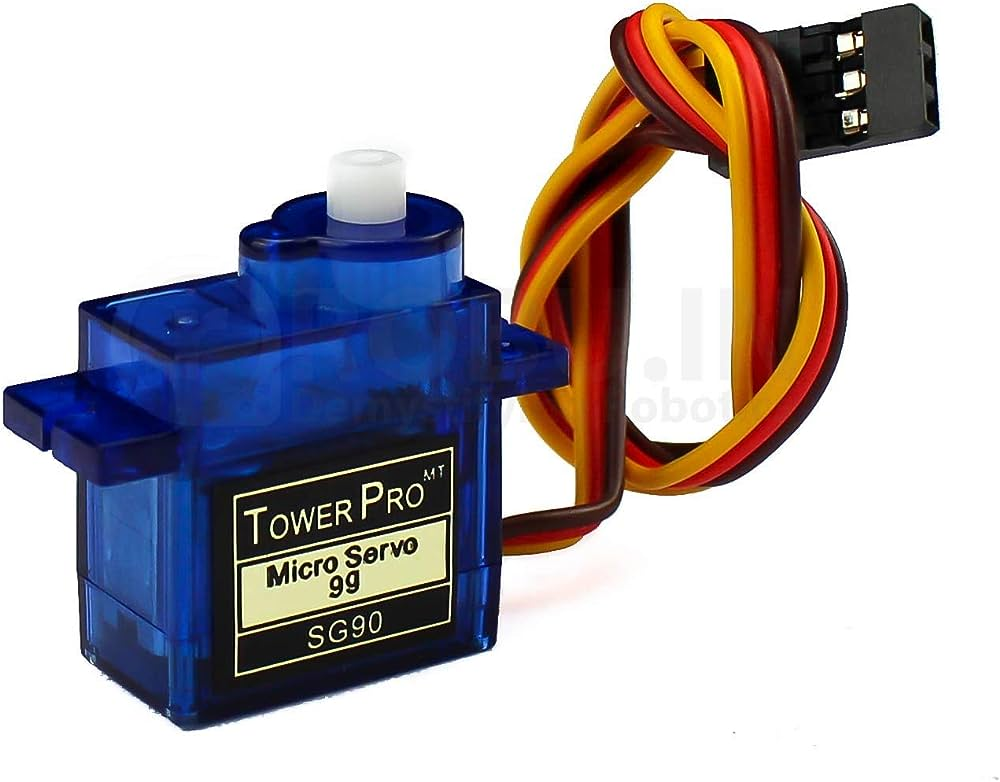
\includegraphics[height=5cm,width=7cm]{./Images/CH3/Servo.jpg}
	\caption{سرو موتور \lr{SG90}}
	\label{سرو موتور}
	\end{figure}

\subsection{اجزای سرو موتور}
یک سرو موتور از سه قسمت اصلی تشکیل شده است:

1. \textbf{موتور}: موتور بسته به منبع تغذیه و نیازهای برنامه کاربردی، ممکن است یک موتور جریان مستقیم
\unskip\LTRfootnote{DC motor}
یا موتور جریان متناوب
\unskip\LTRfootnote{AC motor}
باشد که قدرت مکانیکی را برای چرخش یا حرکت شفت خروجی فراهم می‌کند.

2. \textbf{حسگر}: می‌تواند یک پتانسیومتر، یک انکودر، یک رزولور یا دستگاهی دیگر باشد که موقعیت، سرعت یا گشتاور شفت خروجی را اندازه‌گیری کرده و سیگنال‌های بازخورد را به کنترل‌کننده ارسال می‌کند.

3. \textbf{کنترل‌کننده}: می‌تواند یک مدار آنالوگ یا دیجیتال باشد که سیگنال‌های بازخورد از حسگر را با سیگنال‌های مقدار مورد نظر از یک منبع خارجی (مانند یک کامپیوتر یا یک جوی استیک
\unskip\LTRfootnote{Joystick}
) مقایسه کرده و سیگنال‌های کنترلی را تولید کرده تا ولتاژ یا جریان موتور را به تناسب تنظیم کند. کنترل‌کننده از یک سیستم بازخورد حلقه بسته
\unskip\LTRfootnote{Closed-Loop}
استفاده می‌کند تا حرکت موتور را تنظیم کرده و اطمینان حاصل کند که با مقدار مورد نظر تا حدود خطای مشخصی همخوانی دارد. کنترل‌کننده همچنین می‌تواند از انواع مختلفی از الگوریتم‌های کنترل استفاده کند، مانند کنترل
\lr{PID}
، کنترل منطق فازی
\unskip\LTRfootnote{Fuzzy logic control}
، کنترل تطبیقی
\unskip\LTRfootnote{Adaptive control}
و غیره، به منظور بهینه‌سازی عملکرد موتور سرو.
\subsection{انواع سرو موتور}

موتورهای سرو بر اساس منابع تغذیه، ساختار، مکانیزم بازخورد و کاربردهای خود به انواع مختلفی تقسیم می‌شوند.

1-\textbf{موتورهای سرو جریان متناوب}
\lr{(AC)} 

سرو موتورهای متناوب به دو نوع سنکرون و آسنکرون تقسیم می‌شوند:
\begin{itemize}
\item
سرو موتورهای متناوب سنکرون: دارای یک روتور با آهنربای دائمی هستند که با سرعت مشابه میدان استاتور می‌چرخند. آن‌ها ، دقیق‌تر و پاسخ‌گویی بهتری نسبت به موتورهای آسنکرون دارند، اما به کنترل‌کننده پیچیده‌تری و یک حسگر موقعیت نیاز دارند.
\item
سرو موتورهای متناوب آسنکرون: دارای یک روتور کلافی یا روتور سیم‌پیچی هستند که یک جریان القاء می‌کنند و یک میدان مغناطیسی دارند که عقب‌‌تر از میدان استاتور است. آن‌ها ساده‌تر، ارزان‌تر و مقاوم‌تر از موتورهای سنکرون هستند، اما کارایی، دقت و سرعت پایین‌تری دارند.

سرو موتورهای متناوب برای کاربردهایی با نیاز به توان بالا، سرعت و قابلیت اطمینان مناسب هستند و به طور معمول در دستگاه‌های صنعتی، رباتیک، دستگاه‌های 
\lr{CNC} 
و غیره استفاده می‌شوند.

2-\textbf{موتورهای سرو جریان مستقیم}
\lr{(DC)}

سرو موتورهای جریان مستقیم از جریان مستقیم
\lr{(DC)} 
برای تغذیه خود استفاده می‌کنند. آن‌ها دارای یک استاتور با آهنربای دائمی هستند که یک میدان مغناطیسی ثابت ایجاد می‌کند و یک روتور کلافی دارند که هنگامی که جریانی به آن داده می‌شود، می‌چرخد.

موتورهای سرو جریان مستقیم به دو نوع با جاروبک
\unskip\LTRfootnote{Brushed}
و بدون جاروبک
\unskip\LTRfootnote{Brushless}
 تقسیم می‌شوند.
\item
سرو موتورهای جریان مستقیم با جاروبک: دارای یک کموتاتور
\unskip\LTRfootnote{Commutator}
و جاروبک‌هایی است که جهت جریان را در مارپیچ‌های روتور تغییر می‌دهند. آن‌ها ساده، ارزان و با کنترل آسان هستند، اما به دلیل اصطکاک و سایش تراشه‌ها کارایی، عمر مفید و سرعت پایین‌تری دارند.
\item
سرو موتورهای جریان مستقیم بدون جاروبک: دارای یک کنترل‌کننده الکترونیکی هستند که جهت جریان را در مارپیچ‌های استاتور تغییر می‌دهند. آن‌ها از لحاظ کارایی، مقاومت و سرعت، نسبت به موتورهای تراشه بهتر هستند، اما نیاز به کنترل‌کننده پیچیده‌تر و یک حسگر موقعیت دارند.

سرو موتورهای جریان مستقیم مناسب برای کاربردهای با توان پایین که نیاز به دقت بالا، پاسخگویی و حرکت نرم دارند، هستند و به طور معمول در پروژه‌های سرگرمی، اسباب‌بازی‌های اتومبیل‌، پخش‌کننده‌های
\lr{CD/DVD} 
و غیره استفاده می‌شوند.

در این پروژه برای ساخت ربات چهارپا، با توجه به قابلیت ها و ویژگی ها از موتور جریان مستقیم بدون جاروبک استفاده شده است.
\end{itemize}

\newpage
\section{میکروکنترلر}

میکروکنترلر
\unskip\LTRfootnote{Microcontroller} 
در اصل یک چیپ الکترونیکی برنامه‌پذیر است که با اتصال قطعات مختلف در یک مدار الکترونیکی، اجزای یک کامپیوتر ساده را فراهم می‌کند. از میکروکنترلر برای ساخت، کنترل و مانیتورینگ انواع سیستم‌های الکترونیکی استفاده می‌شود که با برنامه‌ریزی واحدهای میکروکنترلر و تجهیزات جانبی فعال می‌گردد. میکروکنترلر شامل
\lr{CPU}
، حافظه
\lr{RAM/ROM}
، پورت‌های ورودی و خروجی
\lr{(I/O)}
، تایمر، مبدل آنالوگ به دیجیتال
\unskip\LTRfootnote{ADC}
و مبدل دیجیتال به آنالوگ
\unskip\LTRfootnote{DCA}
است.
\lr{CPU}
درواقع همان مغز میکروکنترلر است، که وظیفه‌ی استخراج و پردازش داده ها، انجام محاسبات و وظایف اختصاص­‌داده شده را بر عهده دارد. تایمر برای تولید پالس، اندازه­‌گیری فرکانس و ساخت نوسانات به‌کار می‌رود تا عملیات زمان‌بندی و شمارش را کنترل نماید.

برای برنامه نویسی میکروکنترلر ها ، نرم افزار های خاصی وجود دارند که به آن ها کامپایلر
\unskip\LTRfootnote{Compiler}
می‌گویند. چند تا از کامپایلر های محبوب کیل \lr{(Keil)}، اتمل استودیو \lr{(Atmel Studio)}، کدویژن \lr{(Codevision)} و بسکام \lr{(Bascom)} هستند. 
در هر کامپایلر برنامه نویسی به زبان / زبان های خاصی انجام می‌شود. به طور مثال در کامپایلر کیل از زبان های \lr{C} و اسمبلی (\lr{Assembly}) استفاده می‌شود\cite{Electronics}.


برای استفاده مناسب و صحیح از این قطعه الکترونیکی، باید ابتدا با انواع میکرو کنترلر و کاربردهای آن آشنا شد.

    \begin{figure}[!h]
	\centering
	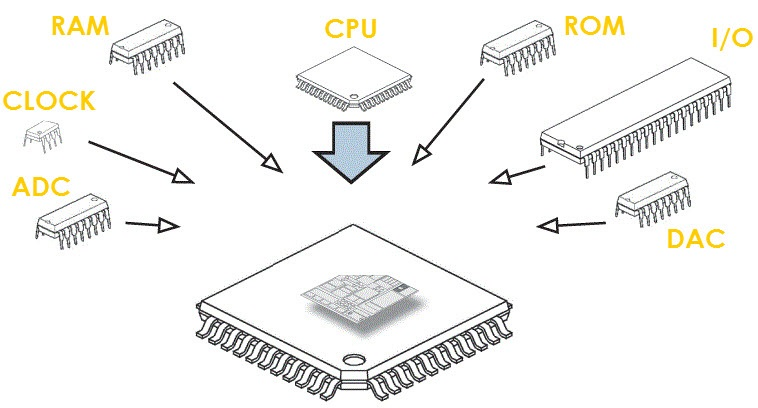
\includegraphics[height=5cm,width=10cm]{./Images/CH3/Micro_Parts.jpg}
	\caption[اجزای میکروکنترلر]{اجزای میکروکنترلر\cite{Micro}}
	\label{اجزا میکرو}
	\end{figure}

\newpage	
\subsection{انواع میکروکنترلر}
اغلب میکروکنترلرها ویژگی‌های مشترک زیادی دارند زیرا همه‌ی آنها دارای یک حافظه درایو، پایه‌های ورودی و خروجی و توان مصرفی کم  هستند. اما در جزِئیاتی مانند تعداد پایه‌ها، ابعاد، قیمت تمام شده و غیره نیز با هم متفاوت‌اند.
میکروکنترلرها براساس حافظه، معماری، بیت‌ها و مجموعه دستورالعمل‌ها به دسته بندی‌های مختلفی تقسیم می‌شوند. در اینجا انواع میکروکنترلرها براساس نوع کارکرد و مداری که در آن ها مورد استفاده قرار می‌گیرند به گروه‌های زیر دسته بندی می‌شوند:
\begin{itemize}
\item
میکروکنترلرهای \lr{AVR}
\item
میکروکنترلرهای  \lr{ARM}
\item
میکروکنترلرهای  \lr{XMEGA}
\item
میکروکنترلرهای  \lr{PIC}
\item
میکروکنترلرهای 8051
\end{itemize}

    \begin{figure}[!h]
	\centering
	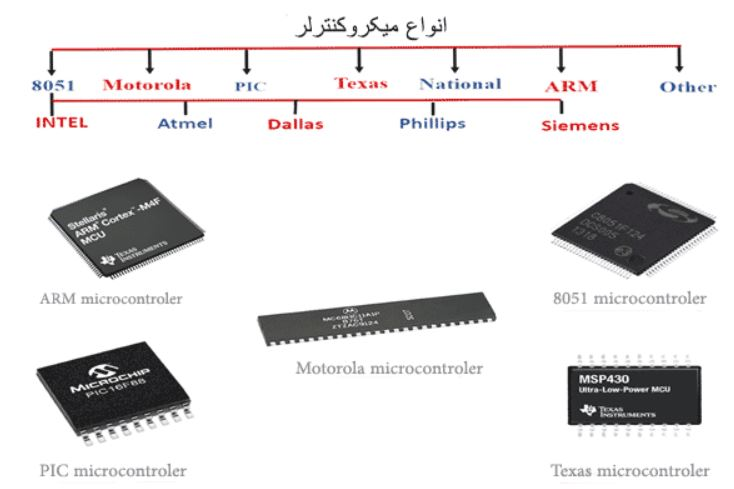
\includegraphics[height=7cm,width=10cm]{./Images/CH3/Micro_Types.JPG}
	\caption[انواع میکروکنترلر]{انواع میکروکنترلر\cite{Micro}}
	\label{انواع میکرو}
	\end{figure}

\newpage
\subsection{مزایا}
ميكروكنترلرها داراي مزاياي متعدد هستند. مزیت فوق العاده میکروکنترلر ها کم شدن تعداد آی‌سی‌ها و قابلیت چند بار نوشتن و پاک کردن کد است.در ذیل چند مزیت مهم میکروکنترلرها آورده شده‌است:

1. \textbf{سهولت برنامه‌نویسی}: ميكروكنترلرها با زبان‌هاي برنامه‌نويسي ساده و قابل فهم برنامه‌ريزي مي‌شوند.

2. \textbf{حجم کم}: ابعاد كوچك ميكروكنترلرها، امكان استفاده در دستگاه‌هاي با اندازه کوچک را فراهم مي‌كند.

3. \textbf{مصرف انرژی پایین}: ميكروكنترلرها از انرژي كمي براي عملكرد خود استفاده مي‌كنند.

4. \textbf{انعطاف‌پذيري}: اين دستگاه‌ها قابليت تغيير برنامه‌هاي خود را دارا هستند و مي‌توان آن‌ها را براي بسياري از كاربردها برنامه‌ريزي كرد.

5. \textbf{هزينه پايين}: ميكروكنترلرها به صورت معمول به صورت اقتصادي قابل تهيه هستند و در اكثر موارد ارزان‌ترين گزينه براي كنترل دستگاه‌ها هستند.

6. \textbf{سرعت بالا}: اين دستگاه‌ها با سرعت بالايي عمل مي‌كنند و گاهی نياز به پردازش سريع دارند.

7. \textbf{قابليت ارتباطات}: ميكروكنترلرها قابليت ارتباط با ساير دستگاه‌هاي الكترونيكي را فراهم مي‌كنند.

8. \textbf{پايداري}: اين دستگاه‌ها داراي پايداري و اطمينان بالايي در عملكرد خود هستند.

با توجه به اين مزايا، ميكروكنترلرها ابزاري قدرتمند براي كنترل و اتوماسيون در صنايع و كاربردهاي الكترونيكي هستند.

\subsection{کاربرد}
همان‌طور که اشاره شد، میکروکنترلر در اصل یک رایانه بسیار کوچک است که در هر پروژه و دستگاهی به طور همزمان نقش قلب و مغز مجموعه را ایفا می‌کند. بنابراین در حال حاضر در بیشتر لوازم خانگی و دستگاه‌های پزشکی و صنعتی مانند سیستم کنترل روشنایی، سیستم کنترل دما و آتش، سیستم‌های کنترل فرمان که در آنها اعمالی همچون اندازه‌گیری، ذخیره‌سازی، محاسبه، کنترل و نمایش اطلاعات انجام می‌شود، از میکروکنترلر استفاده شده است. 
    \begin{figure}[!h]
	\centering
	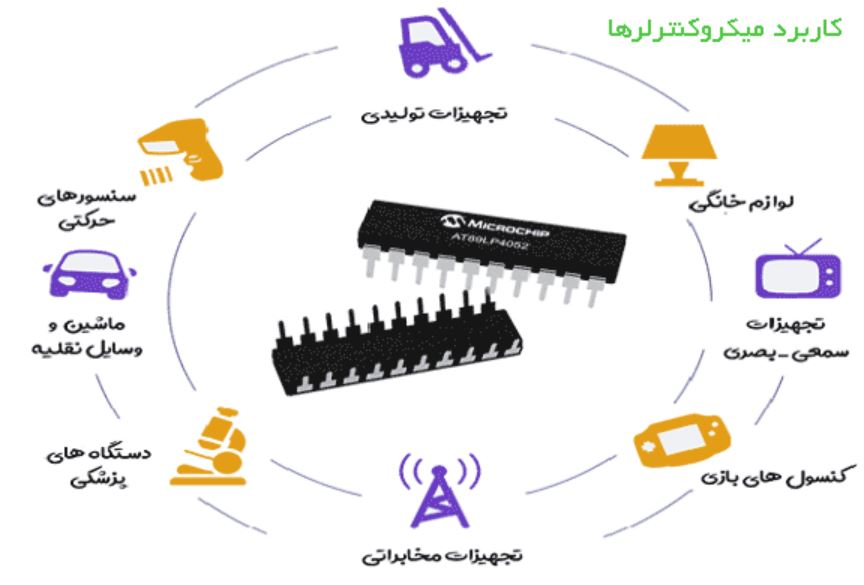
\includegraphics[height=4cm,width=8cm]{./Images/CH3/Micro_Uses.JPG}
	\caption[کاربردهای میکروکنترلر]{کاربردهای میکروکنترلر\cite{Micro}}
	\label{کاربرد میکرو}
	\end{figure}

با توجه به تمام نکات در ابتدا قصد به استفاده از ماژول \lr{Arduino Uno} داشتیم اما به این دلیل که ما برای کنترل هر موتور به یک پایه با قابلیت \lr{PWM} نیاز داریم تصمیم به استفاده از ماژول \lr{STM32F103C8T6} گرفتیم که تمام خواسته‌های ما را برطرف می‌کند.
\section{ماژول \lr{STM32F103C8T6}}
میکروکنترلر \lr{STM32F103C8T6} دارای هسته پردازنده 32 بیتی\lr{ARM Cortex M3 } توسط شرکت \lr{STMicroelectronics} ساخته شده است است. این برد شامل میکروکنترلر \lr{STM32F103C8T6}، پورت میکرو \lr{USB} تغذیه، دکمه \lr{Reset}، دو سلکتور \lr{BOOT0} و \lr{BOOT1}، کریستال \lr{8MHz}، کریستال \lr{RTC 32.768KHz}، دو \lr{LED} (یک \lr{LED} نمایش دهنده اتصال تغذیه و دیگری متصل به پین \lr{C13} برای استفاده کاربر)، رگولاتور \lr{3.3V} و هدر برد پایه‌های \lr{SWI} برای پروگرام کردن میکرو است.

مشخصات فنی ماژول موردنظر:
\begin{itemize}
	\item دارای هسته 32 بیتی \lr{ARM Cortex M3}
	\item ولتاژ کاری: 7.2 تا 6.3 ولت
	\item فرکانس: ماکزیمم 72 مگاهرتز
	\item حافظه: 64 کیلوبایت
	\item تعداد پین‌های ورودی/خروجی: 37
	\item تعداد پین‌های \lr{PWM}: 4 + 12
	\item تایمر: 3+1
	\item پروتکل های ارتباطی: \lr{I2C, SPI, UART/USART}
\end{itemize}

    \begin{figure}[!h]
	\centering
	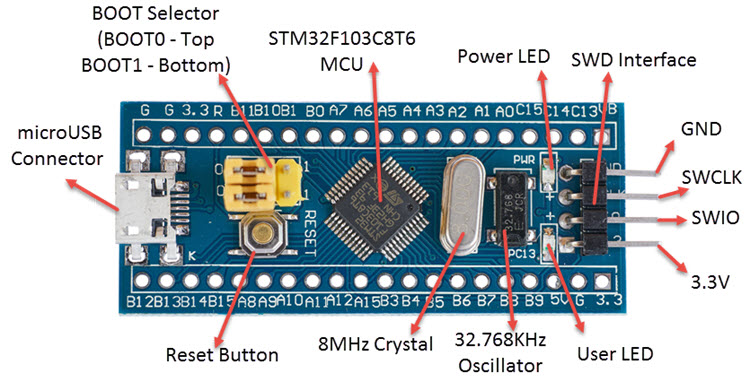
\includegraphics[height=4.9cm,width=9cm]{./Images/CH3/STM32.jpg}
	\caption{ماژول \lr{STM32F103C8T6}}
	\label{STM32}
	\end{figure} 

\section{ماژول \lr{Arduino-Uno}}

برد  \lr{Arduino Uno}، یک برد متن‌باز مبتنی بر میکروکنترلر   \lr{Microchip ATmega328P} است و توسط شرکت \lr{Arduino.cc} ساخته شده است. این برد مجهز به مجموعه‌ای از پین‌های ورودی / خروجی دیجیتال و آنالوگ است که می‌تواند به راحتی با شیلدهای آردوینو ارتباط برقرار کند. برد \lr{Uno} اولین سری از سری برد های آردوینو مبتنی بر \lr{USB} است. میکروکنترلر \lr{ATmega328} موجود در برد با یک بوت لودر از قبل برنامه ریزی شده است که اجازه می دهد بدون استفاده از پروگرمر سخت افزاری خارجی برنامه‌ریزی شود. ماژول آردوینو اونو در زیر آورده شده است:

    \begin{figure}[!h]
	\centering
	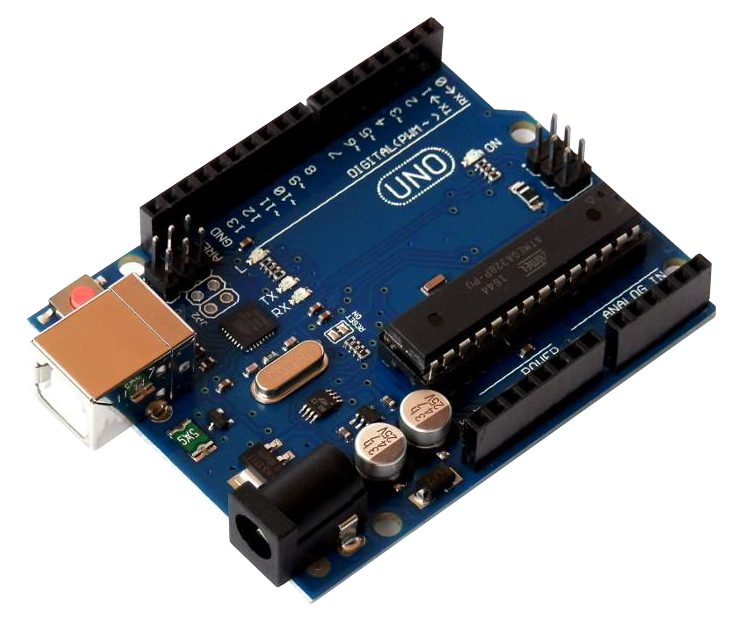
\includegraphics[height=5cm,width=8cm]{./Images/CH3/Arduino_Uno.png}
	\caption{ماژول \lr{Arduino Uno}}
	\label{Arduino}
	\end{figure} 
برای پروگرم کردن ماژول \lr{ESP32-CAM} نیاز داریم که با استفاده از پروتکل سریال این کار را انحام دهیم و برای انجام آن از \lr{FTDI} استفاده می‌کنیم که رابط سریال به \lr{USB} می‌باشد. اما ما به‌جای آن از ماژول \lr{Arduino Uno} استفاده می‌کنیم هم به دلیل دردسترس بودن، سادگی و توانایی مشاهده اطلاعاتی که از دوربین برای ما فرستاده می‌شود؛ مانند متصل بودن یا نبودن به روتر و \lr{IP} که دوربین روی آن بالا آمده‌است.
\section{ماژول \lr{ESP32-CAM}}

ماژول \lr{ESP32-CAM} یک ماژول کامل با میکروکنترلری یکپارچه است که می‌تواند به‌طور مستقل کار کند. علاوه بر اتصال اینترنت و بلوتوث، دارای یک دوربین فیلمبرداری یکپارچه و یک کارت حافظه \lr{microSD} برای ذخیره سازی است. این قطعه برای نظارت و شناسایی تصویر بسیار کاربردی است.

مشخصات فنی این ماژول به شرح زیر است:
\begin{itemize}
\item 
ارتباطات: بلوتوث \lr{BLE 4.2} به همراه \lr{WiFi 802.11b}. که از بارگذاری تصویر از طریق \lr{WiFi} پشتیبانی می کند.
\item
اتصالات: \lr{UART} ، \lr{SPI} ، \lr{I2C}، و \lr{PWM} و دارای 9 پایه \lr{GPIO} است.
\item
فرکانس کاری: تا 160 مگاهرتز
\item
حافظه: 520 کیلوبایت \lr{SRAM}، چهار مگابایت حافظه کارت \lr{PSRAM + SD}
\item
دوربین: از دوربین های \lr{OV2640} پشتیبانی می‌کند که دارای 2 مگاپیکسل روی سنسور با اندازه آرایه  1622 × 1200\lr{UXGA} پیکسل هستند.
\end{itemize}

    \begin{figure}[!h]
	\centering
	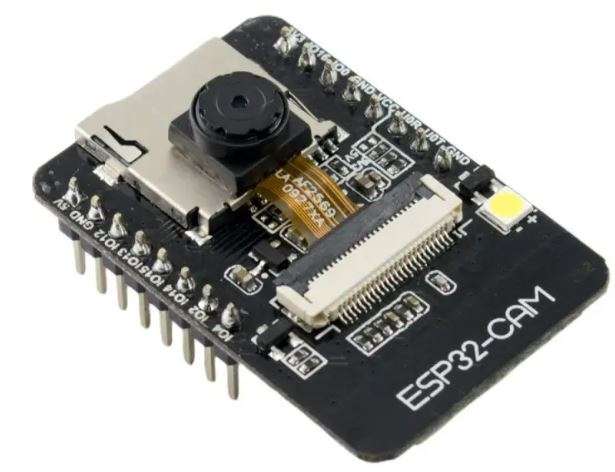
\includegraphics[height=4.3cm,width=6cm]{./Images/CH3/ESP32CAM.jpg}
	\caption{ماژول \lr{ESP32-CAM}}
	\label{ESP32}
	\end{figure} 

\section{منبع تغذیه دی سی}

منبع تغذیه را می‌توان اینگونه تعریف کرد که یک وسیله الکتریکی است که برای تامین برق بارهای الکتریکی استفاده می شود. وظیفه اصلی این دستگاه تغییر جریان الکتریکی از منبع به ولتاژ، فرکانس و جریان دقیق برای تامین بار می‌باشد. منبع تغذیه دی‌سی
\lr{DC}
\unskip\LTRfootnote{Direct Current}
 منبع تغذیه ای است که ولتاژ دی‌سی ثابتی را برای بار خود فراهم می‌کند. منبع تغذیه \lr{DC} که به عنوان منبع تغذیه میزی نیز شناخته می‌شود، نوعی منبع تغذیه است که ولتاژ جریان مستقیم \lr{(DC)} را برای تغذیه یک دستگاه تامین می‌کند.
 
 در این پروژه، علت استفاده از منبع ولتاژ دی‌سی به جای باتری، کاهش وزن ربات، توان خروجی بالا و عملکرد پایدارتر است. 
 
    \begin{figure}[!h]
	\centering
	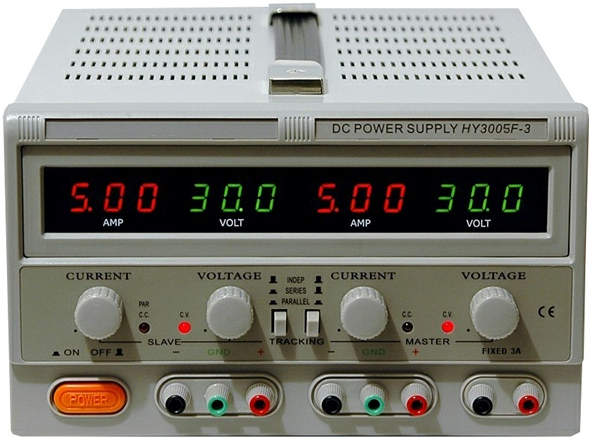
\includegraphics[height=4cm,width=7cm]{./Images/CH3/DC_supply.png}
	\caption{منبع ولتاژ \lr{DC}}
	\label{منبع ولتاژ}
	\end{figure} 

\section{برد الکترونیکی}

بردهای الکترونیکی شامل \lr{Breadboard}، برد مدارچاپی 
\unskip\LTRfootnote{PCB}
و برد‌ 1000 سوراخ
\unskip\LTRfootnote{Stripboard}
هستند. این ابزارها به عنوان پایه‌هایی برای ساخت و اتصال مدارهای الکترونیکی عمل می‌کنند و در جنبه‌های عملکردی متفاوتی دارند. در زیر توضیح مختصری از هرکدام ارائه شده است:

\subsection{\lr{Breadboard}}
بردبورد وسیله‌ای است که می‌توان با استفاده از آن بدون لحیم کاری نمونه‌های اولیه مدارهای الکترونیکی را طراحی و تست نمود. با قرار دادن پایه های قطعات الکترونیکی در سوراخ ها و سپس برقراری اتصال به وسیله سیم در مدار های الکترونیکی به یکدیگر وصل می‌شوند. بردبورد نوارهای فلزی دارد که در زیر سوراخ‌های پلاستیکی قرار گرفته و آن‌ها را به هم متصل می‌کند. سوراخ‌های ردیف‌های بالا و پایین به صورت افقی متصل هستند و به وسیله شیاری در وسط تقسیم می‌شوند در حالی که سوراخ‌های باقی مانده به صورت عمودی متصل هستند.
    \begin{figure}[!h]
	\centering
	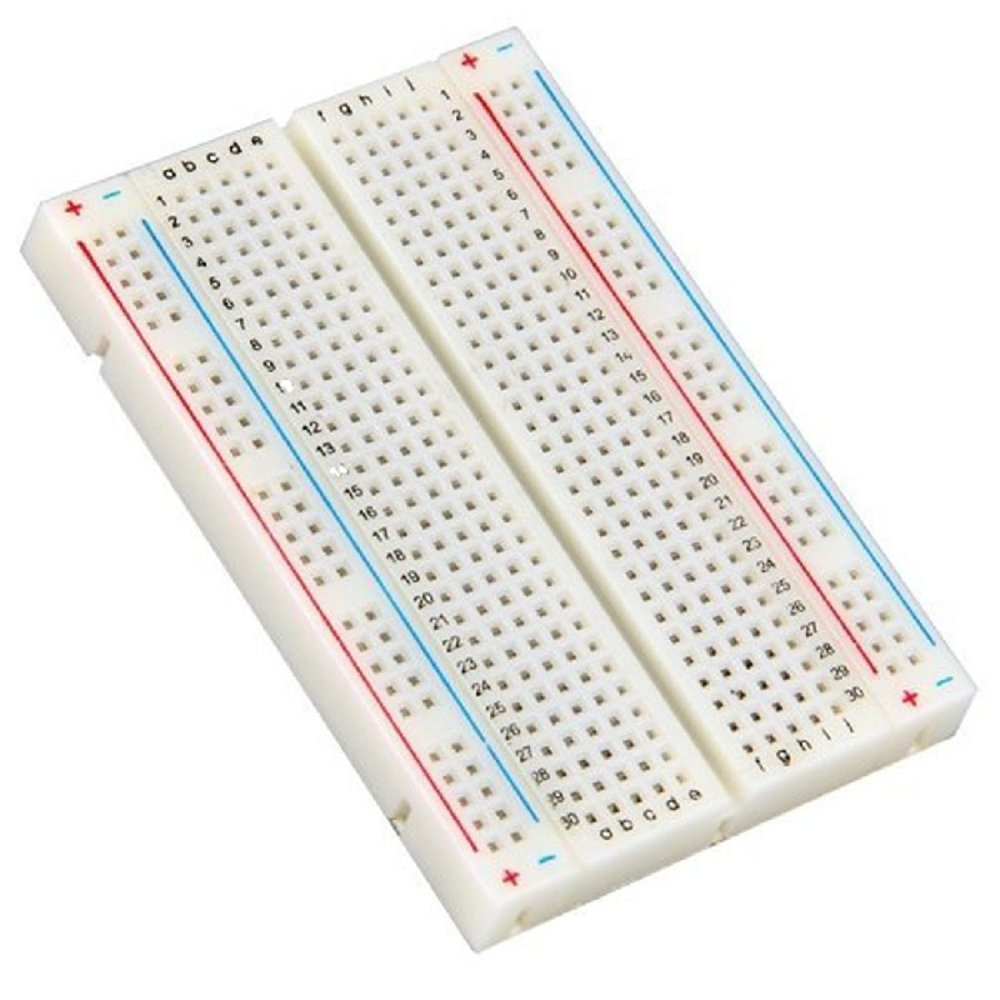
\includegraphics[height=5cm,width=6cm]{./Images/CH3/Breadboard.jpg}
	\caption{\lr{Breadboard}}
	\label{برد بورد}
	\end{figure} 
\subsection{برد \lr{PCB}}

برد مدار چاپی یا \lr{PCB}
\unskip\LTRfootnote{Printed Circuit Board}
یک برد  غیررسانا و چندلایه مسی است که تمامی قطعات الکتریکی و الکترونیکی از طریق یک برد مشترک و به‌وسیله تکیه‌گاه فیزیکی نصب شده در کف برد به یکدیگر متصل‌اند. قبل از رشد و گسترش بردهای مدار چاپی، مدار ها به‌وسیله سیم‌کشی نقطه به نقطه ساخته می شدند که باعث افزایش پیچیدگی و عدم اطمینان در مدار می‌شد. در نتیجه هیچ‌گاه (بوسیله اتصال قطعات با سیم) قادر به ساخت مدار بزرگی نبودیم. در برد مدار چاپی تمامی قطعات بدون سیم و از داخل به یکدیگر متصل‌اند که این ویژگی منجر به کاهش پیچیدگی طرح کلی مدار می‌شود.روش طراحی \lr{PCB} به گونه‌ای است که  در فراهم کردن الکتریسیته و اتصال بین قطعات مدار کاربرد ویژه‌‌ای دارد.

    \begin{figure}[!h]
	\centering
	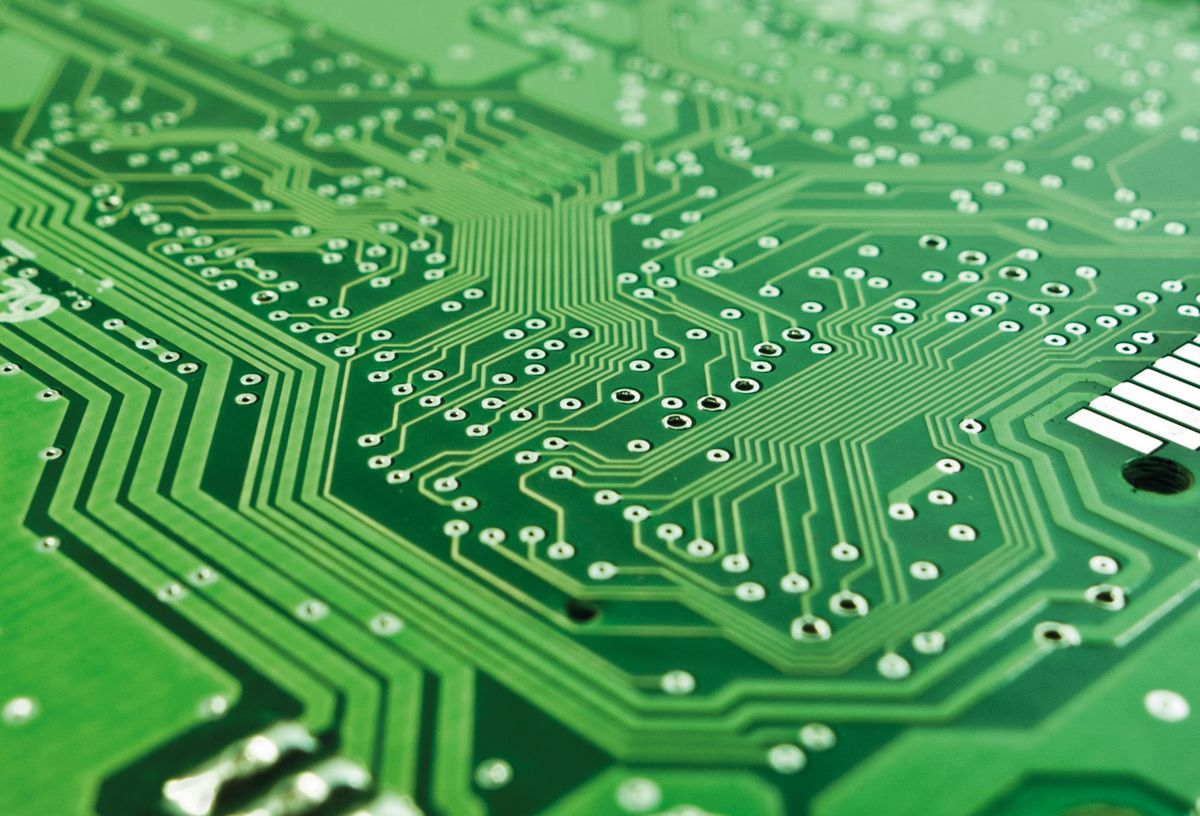
\includegraphics[height=4.5cm,width=7cm]{./Images/CH3/PCB.jpg}
	\caption{یک نمونه برد مدار چاپی}
	\label{مدار چاپی}
	\end{figure} 

\subsection{هزار سوراخ}

برد هزار سوراخ‌
\unskip\LTRfootnote{Stripboard}
گزینه دیگری است که می‌توان هنگام ساخت برد مدار برای پروژه الکترونیکی در نظر گرفت. این بردها برای نمونه‌سازی و تولید بردهای مدارهای کاربردی عالی هستند.بردهای هزار سوراخ با سوراخ‌های مشبک مستطیلی 0.1 اینچی و نوارهای مسی موازی در یک طرف مشخص می‌شوند. قطعات الکترونیکی باید روی این بردها لحیم شوند. با توجه به سوراخ 0.1 اینچی، به قطعاتی با پین‌های 0.1  اینچی نیاز است. قطعات همیشه در یک طرف بورد قرار می‌گیرند، در حالی که انتهای پایه آ‌ن‌ها در انتهای دیگر بیرون می‌آید. سپس محل برخورد برد و پایه قطعات باید لحیم شوند. لحیم‌کاری باید به‌گونه‌ای باشد که اطمینان حاصل شود که پایه‌ها به مسیرهای مسی در طرف دیگر نوار وصل هستند. در مواردی که نیاز به اتصال سیم است، استفاده از سیم‌های 0.1 اینچی توصیه می‌شود. بردهای هزار سوراخ برای ساخت مدارهای کوچک عالی هستند اما محدودیت‌هایی نیز دارند.

    \begin{figure}[!h]
	\centering
	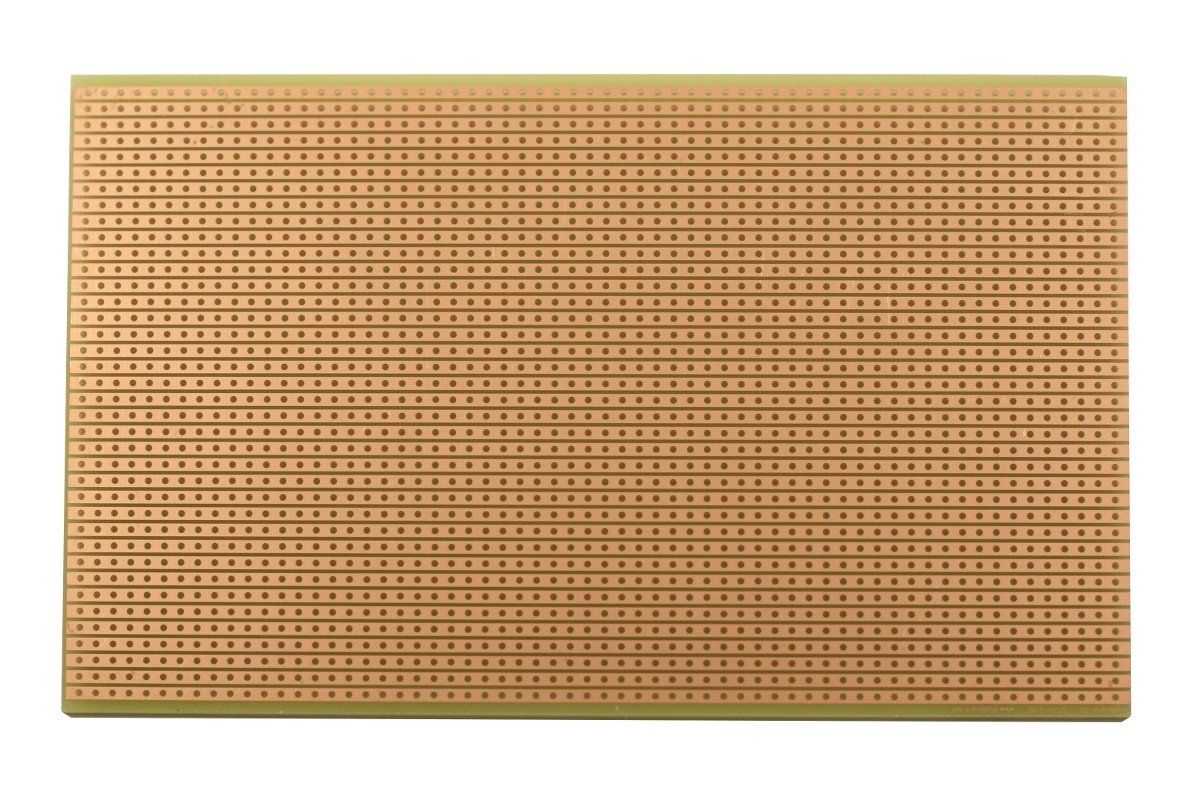
\includegraphics[height=4.9cm,width=6.5cm]{./Images/CH3/Stripboard.jpg}
	\caption{یک نمونه برد هزار سوراخ}
	\label{برد هزار سوراخ}
	\end{figure} 
	
	در این پروژه، با توجه به بودجه مالی و امکانات، استفاده از برد هزار سوراخ بهترین گزینه ممکن است.

\section{جمع بندی}
با بررسی تمام نکات و نیازهای ما برای انجام هرچه بهتر این پروژه، درنهایت بهترین انتخاب برای هر قطعه را با توجه به محدودیت مالی و زمانی انجام دادیم. نکته بسیار مهم که در آخر باید به آن اشاره شود این است که به این مسئله که آیا تمام قطعات با یکدیگر می‌توانند کار کنند و همان عملکری که از آن‌ها توقع داریم را برآورده کنند یا خیر. به عنوان مثال ما در ابتدا قصد استفاده از \lr{Arduino Uno} داشتیم اما به دلیل نیاز به 12 پایه با قابلیت \lr{PWM} از ماژول \lr{STM32F103C8T6} استفاده کردیم.